\begin{figure}[H]
    \centering
    \definecolor{benzeneblue}{RGB}{92,185,220}
    \definecolor{gasorange}{RGB}{250,225,180}
    \definecolor{pressureblue}{RGB}{35,95,170}
    \definecolor{pressurered}{RGB}{190,45,45}
    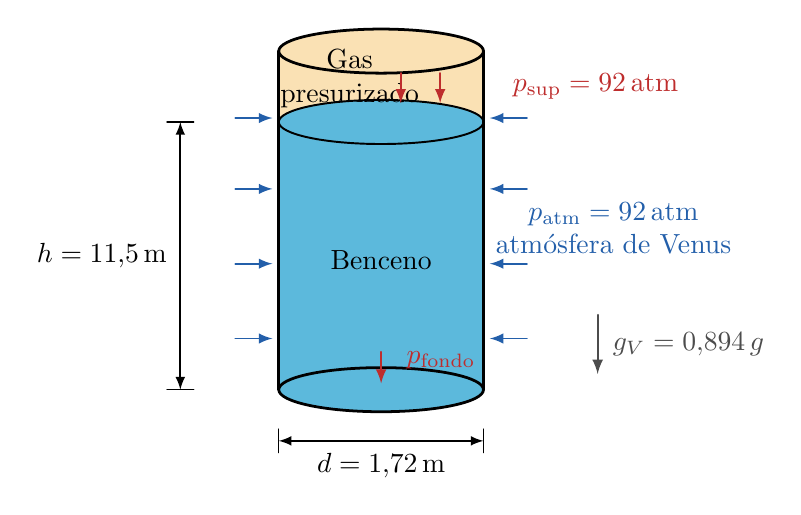
\begin{tikzpicture}[x=1cm,y=1cm,line cap=round,line join=round]
        \def\xL{2.60}
        \def\xR{5.20}
        \def\xC{3.90}
        \def\yB{0.70}
        \def\yS{4.10}
        \def\yT{5.00}
        \def\rx{1.30}
        \def\ry{0.28}

        % Fases en el interior del tanque
        \fill[gasorange] (\xL,\yS) rectangle (\xR,\yT);
        \fill[gasorange] (\xC,\yT)
            ellipse [x radius=\rx,y radius=\ry];
        \fill[benzeneblue] (\xL,\yB) rectangle (\xR,\yS);
        \fill[benzeneblue] (\xC,\yB)
            ellipse [x radius=\rx,y radius=\ry];
        \fill[benzeneblue] (\xC,\yS)
            ellipse [x radius=\rx,y radius=\ry];

        % Pared y tapas del tanque cilíndrico
        \draw[line width=1.0pt] (\xL,\yB) -- (\xL,\yT);
        \draw[line width=1.0pt] (\xR,\yB) -- (\xR,\yT);
        \draw[line width=1.0pt] (\xC,\yT)
            ellipse [x radius=\rx,y radius=\ry];
        \draw[line width=1.0pt] (\xC,\yB)
            ellipse [x radius=\rx,y radius=\ry];

        % Superficie libre del benceno
        \draw[line width=0.7pt] (\xC,\yS)
            ellipse [x radius=\rx,y radius=\ry];
        \node at (\xC,2.35) {Benceno};
        \node[align=center] at (3.50,4.65) {Gas\\presurizado};

        % Presión interna aplicada sobre la superficie del líquido
        \foreach \x in {4.15,4.65} {
            \draw[pressurered,-latex,line width=0.75pt]
                (\x,4.72) -- (\x,4.34);
        }
        \node[pressurered,right] at (5.45,4.55)
            {$p_{\mathrm{sup}}=92\,\mathrm{atm}$};

        % Presión atmosférica exterior sobre las paredes verticales
        \foreach \y in {1.35,2.30,3.25,4.15} {
            \draw[pressureblue,-latex,line width=0.70pt]
                (2.05,\y) -- (2.52,\y);
            \draw[pressureblue,-latex,line width=0.70pt]
                (5.75,\y) -- (5.28,\y);
        }
        \node[pressureblue,align=center] at (6.85,2.75)
            {$p_{\mathrm{atm}}=92\,\mathrm{atm}$\\atmósfera de Venus};

        % Altura de la columna de benceno
        \draw[latex-latex,line width=0.6pt] (1.35,\yB) -- (1.35,\yS);
        \draw[line width=0.45pt] (1.18,\yB) -- (1.52,\yB);
        \draw[line width=0.45pt] (1.18,\yS) -- (1.52,\yS);
        \node[left,align=center] at (1.30,2.40) {$h=11{,}5\,\mathrm{m}$};

        % Diámetro interior
        \draw[latex-latex,line width=0.6pt] (\xL,0.05) -- (\xR,0.05);
        \draw[line width=0.45pt] (\xL,-0.10) -- (\xL,0.20);
        \draw[line width=0.45pt] (\xR,-0.10) -- (\xR,0.20);
        \node[below] at (\xC,0.02) {$d=1{,}72\,\mathrm{m}$};

        % Gravedad de Venus
        \draw[black!70,-latex,line width=0.8pt]
            (6.65,1.65) -- (6.65,0.90);
        \node[black!70,right] at (6.72,1.28)
            {$g_V=0{,}894\,g$};

        % Presión en el fondo usada en el inciso (a)
        \draw[pressurered,-latex,line width=0.75pt]
            (\xC,1.18) -- (\xC,0.78);
        \node[pressurered,right] at (4.10,1.08) {$p_{\mathrm{fondo}}$};
    \end{tikzpicture}
    \caption{Tanque cilíndrico presurizado con benceno en Venus.}
\end{figure}
